\subsection{Shell-Sort Algorithm:}

First test of {\bfseries Shell-Sort} algorithm. The program will plot the time that the algorithm takes to sort three lists of size {\itshape n = 10}. The first list will have the elements already sorted, the second will have the elements in random order, and the third list will have the elements sorted but in decreasing order. With this we will corroborate the complexity of this algorithm presented in section 2. Each list represents its {\itshape best, random and worst} case. \hfill \break

\begin{figure}[H]
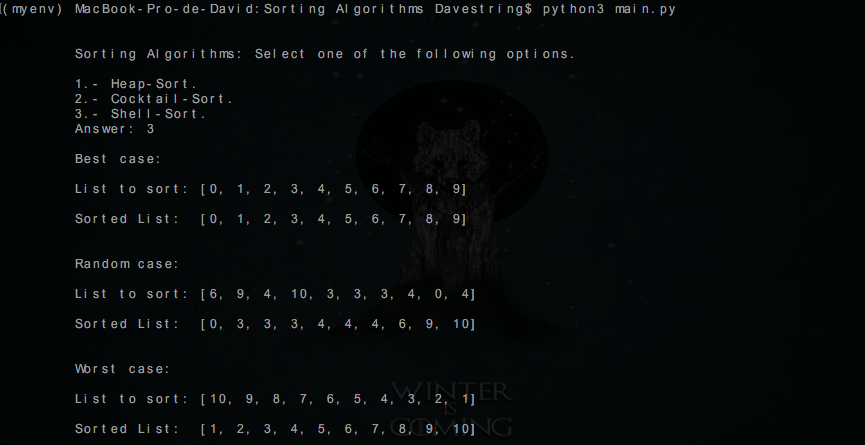
\includegraphics[width = 16.5cm, height = 8cm]{Shell-output-10.png}
\centering \linebreak \linebreak {\small Figure 4.3.0: Shell-Sort console output.}
\end{figure}

\begin{figure}[H]
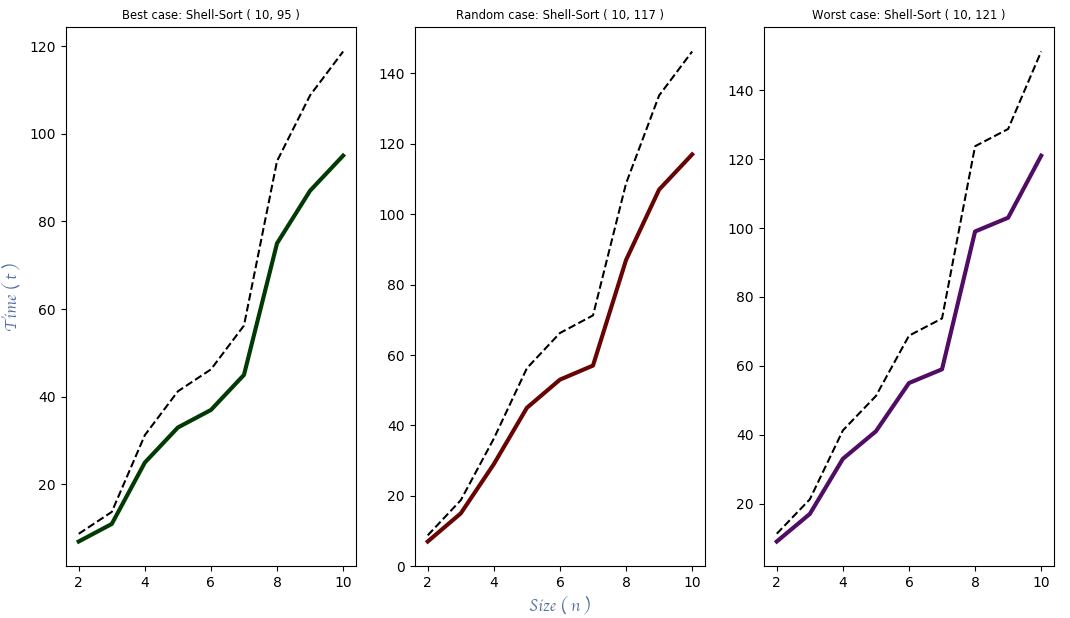
\includegraphics[width = 16.5cm, height = 8cm]{Shell-10.png}
\centering \linebreak \linebreak {\small Figure 4.3.1: Shell-Sort graph for the lists in Figure 4.3.0.}
\end{figure} \pagebreak

Table 5 illustrate the plotting points of Figure 4.3.1 graphs, the first column represents the size of the list to sort, the second, third and fourth, the time that takes to sort that list in its best, random and worst case of the algorithm. \hfill \break

{\small
\begin{center} 
\begin{tabular}[.5cm]{ c c c c } 
\toprule \toprule
\hspace {5px} Size ( n ) \hspace {5px} & \hspace {15px} Best Case Time ( t ) \hspace {15px} & \hspace {15px} Random Case Time ( t ) \hspace {15px} & \hspace {15px} Worst Case Time ( t ) \hspace {15px} \\ 
\midrule \midrule
2 & 7 & 7 & 9 \\ 
\cmidrule {1-4} 
3 & 11 & 15 & 17 \\ 
\cmidrule {1-4} 
4 & 25 & 29 & 33 \\ 
\cmidrule {1-4} 
5 & 33 & 45 & 41 \\ 
\cmidrule {1-4} 
6 & 37 & 53 & 55 \\ 
\cmidrule {1-4} 
7 & 45 & 57 & 59 \\ 
\cmidrule {1-4} 
8 & 75 & 87 & 99 \\ 
\cmidrule {1-4} 
9 & 87 & 107 & 103 \\ 
\cmidrule {1-4} 
10 & 95 & 117 & 121 \\ 
\bottomrule 
\linebreak 
\end{tabular} 
\linebreak \linebreak Table 5.
\end{center}}

{\bfseries\itshape\color{carmine}{Observation:}} {\itshape\color{carmine}{In Figure 4.3.1 there are 3 graphs, the one on the left represent the algorithm's best case, analogously the middle and right ones represents the random and worst case, in each graph, there is a {\bfseries pointed} stroke, this it's an asymptotic function for the main plot.}}

\pagebreak

Second test of {\bfseries Shell-Sort} algorithm. The program will plot the time that the algorithm takes to sort three lists of size {\itshape n = 20}. The first list will have the elements already sorted, the second will have the elements in random order, and the third list will have the elements sorted but in decreasing order. With this we will corroborate the complexity of this algorithm presented in section 2. Each list represents its {\itshape best, random and worst} case. \hfill \break

\begin{figure}[H]
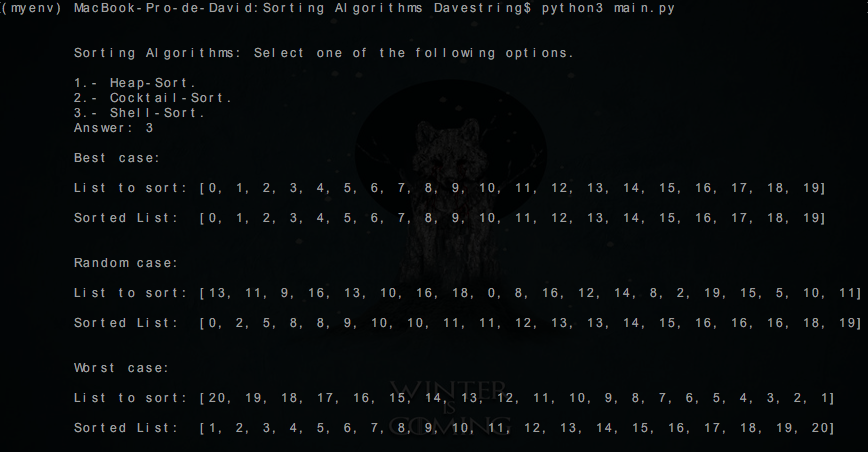
\includegraphics[width = 16.5cm, height = 8cm]{Shell-output-20.png}
\centering \linebreak \linebreak {\small Figure 4.3.2: Shell-Sort console output.}
\end{figure}

\begin{figure}[H]
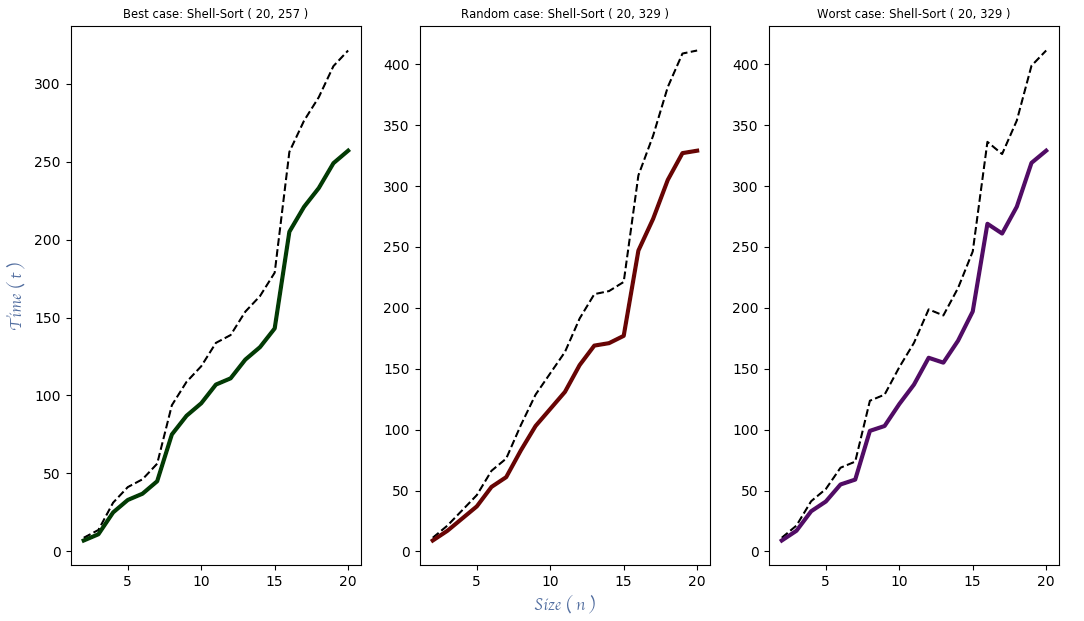
\includegraphics[width = 16.5cm, height = 8cm]{Shell-20.png}
\centering \linebreak \linebreak {\small Figure 4.3.3: Shell-Sort graph for the lists in Figure 4.3.2.}
\end{figure} \pagebreak

Table 6 illustrate the plotting points of Figure 4.3.3 graphs, the first column represents the size of the list to sort, the second, third and fourth, the time that takes to sort that list in its best, random and worst case of the algorithm. \hfill \break

{\small
\begin{center} 
\begin{tabular}[.5cm]{ c c c c } 
\toprule \toprule
\hspace {5px} Size ( n ) \hspace {5px} & \hspace {15px} Best Case Time ( t ) \hspace {15px} & \hspace {15px} Random Case Time ( t ) \hspace {15px} & \hspace {15px} Worst Case Time ( t ) \hspace {15px} \\ 
\midrule \midrule
2 & 7 & 9 & 9 \\ 
\cmidrule {1-4} 
3 & 11 & 17 & 17 \\ 
\cmidrule {1-4} 
4 & 25 & 27 & 33 \\ 
\cmidrule {1-4} 
5 & 33 & 37 & 41 \\ 
\cmidrule {1-4} 
6 & 37 & 53 & 55 \\ 
\cmidrule {1-4} 
7 & 45 & 61 & 59 \\ 
\cmidrule {1-4} 
8 & 75 & 83 & 99 \\ 
\cmidrule {1-4} 
9 & 87 & 103 & 103 \\ 
\cmidrule {1-4} 
10 & 95 & 117 & 121 \\ 
\cmidrule {1-4} 
11 & 107 & 131 & 137 \\ 
\cmidrule {1-4} 
12 & 111 & 153 & 159 \\ 
\cmidrule {1-4} 
13 & 123 & 169 & 155 \\ 
\cmidrule {1-4} 
14 & 131 & 171 & 173 \\ 
\cmidrule {1-4} 
15 & 143 & 177 & 197 \\ 
\cmidrule {1-4} 
16 & 205 & 247 & 269 \\ 
\cmidrule {1-4} 
17 & 221 & 273 & 261 \\ 
\cmidrule {1-4} 
18 & 233 & 305 & 283 \\ 
\cmidrule {1-4} 
19 & 249 & 327 & 319 \\ 
\cmidrule {1-4} 
20 & 257 & 329 & 329 \\ 
\bottomrule 
\linebreak 
\end{tabular} 
\linebreak \linebreak Table 6.
\end{center}}

\pagebreak

Our last test for this algorithm consist in plotting the complexity of lists of sizes {\itshape n = 10000} as we can see in Figure 4.3.4. In this examples we can visualize that the algorithm in its best case is near to {\bfseries $\mathcal{O}(n)$}, otherwise {\bfseries $\mathcal{O}(n^{\frac{3}{2}})$ or $\mathcal{O}(n\log^{2}(n))$} time depending of the gap. \hfill \break

\begin{figure}[H]
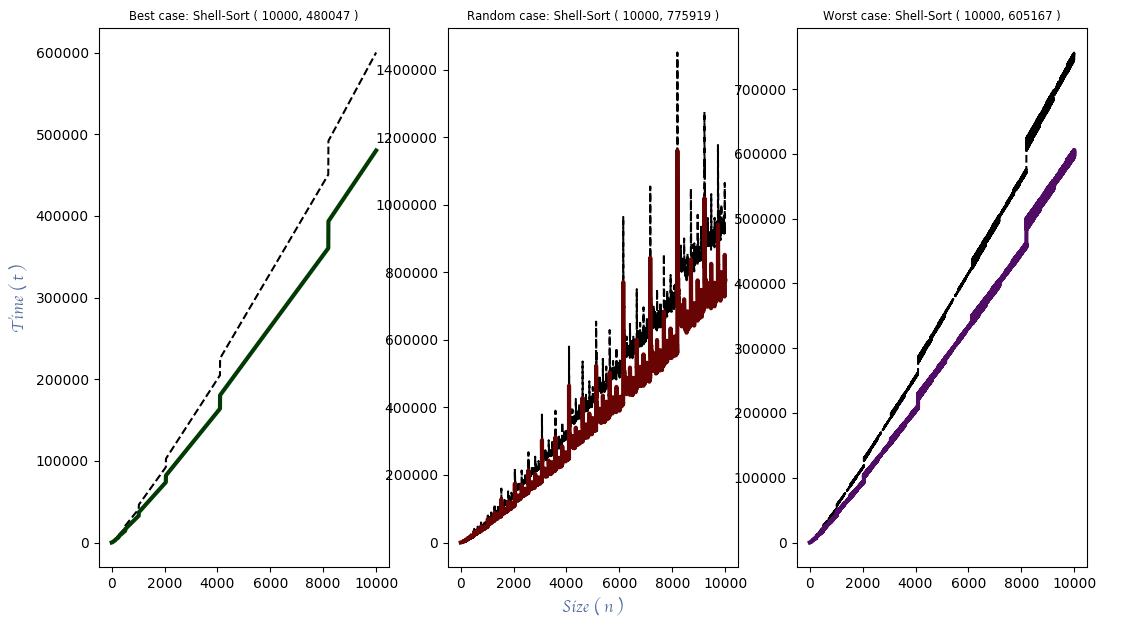
\includegraphics[width = 16.5cm, height = 8cm]{Shell-10000.png}
\centering \linebreak \linebreak {\small Figure 4.3.4: Shell-Sort complexity for lists of size n = 10000.}
\end{figure}

{\bfseries\itshape\color{carmine}{Observation:}} {\itshape\color{carmine}{In Figure 4.3.4 we can visualize that the middle and right plots are something strange, I've been researching and this algorithm doesn't have an exact superior asymptotic function, the running time depends of how the programmer assign something know as {\bfseries gap}, still, this algorithm is under $\mathcal{O}(n^{2})$ and this, makes it better than {\bfseries Insertion-Sort}.}}

\pagebreak